\chapter{Introdução}

O termo Internet das Coisas, do inglês, \textit{Internet of Things} (IoT), foi usado pela primeira vez em 1998 para definir objetos do mundo físico representados virtualmente por meio de dispositivos interconectados~\cite{weber2010internet}. 

Advinda do avanço das áreas de sistemas embarcados, microeletrônica, comunicação e tecnologia de informações ~\cite{iot2016}, a IoT é considerada uma das mais promissoras tecnologias emergentes~\cite{gartner2015gartner}. Em estudo realizado pela \textit{Acquity Group}, mais de dois terços dos consumidores planejam comprar tecnologia conectada para suas casas até 2019~\cite{press2014internet}. Estima-se que, até 2017, 82\% das empresas implementarão a IoT de alguma forma, conforme relatório publicado pela \textit{Business Insider UK}~\cite{danova2014bi}.

%Conforme o crescimento da quantidade de dispositivos e aplicativos conectados a \textit{Internet}, aumenta o interesse dos usuários em adquiri-los, tal como o de empresas em investir neste mercado~\cite{mukherjee2016ranking}.

Por meio da conexão e troca de mensagens entre os dispositivos, é possível realizar o monitoramento de ambientes controlados,  dispondo de uma vasta área de aplicações. Entre elas, pode-se destacar: carros, cidades e fazendas inteligentes; transporte e logística; cuidados médicos; interação pessoal e social; e processos industriais~\cite{sankarinternet, bandyopadhyay2011internet, atzori2010internet}.

Dentre os diversos fatores responsáveis pelo crescimento do interesse na área, ressalta-se a miniaturização do \textit{hardware}, além da criação do Protocolo de \textit{Internet} IPv6~\cite{press2014internet}. Capaz de alocar até $2^{128}$ endereços IP, o IPv6 possibilita a conexão de uma extensa quantidade de dispositivos~\cite{mukherjee2016ranking}.

De forma geral, dispositivos utilizados em IoT possuem recursos limitados de memória e processamento, além de operarem em ambientes com baixa largura de banda ou redes instáveis ~\cite{weber2010internet, iot2016, suo2012security}. Portanto, é essencial que a comunicação e a troca de dados entre eles seja executada da forma eficiente, sendo este, um dos principais desafios enfrentados na área~\cite{bandyopadhyay2011internet, suo2012security}.

Devido as suas características, as aplicações de IoT necessitam de padronizações específicas. Logo, tratando-se estritamente da comunicação entre os dispositivos, foi desenvolvido em 1999 pela IBM e Eurotech o protocolo MQTT (\textit{Message Queue Telemetry Transport protocol})~\cite{mqttv3.1}. 

Padronizado em 2014 pela OASIS~\cite{mqttv3.1.1}, o MQTT tem como principal objetivo minimizar o uso de largura de banda da rede e recursos dos dispositivos. Para isso, o protocolo foi desenvolvido com base em diversos conceitos que asseguram uma alta taxa de entrega das mensagens~\cite{chen2014responsive}.

A comunicação é crucial para a execução correta de um sistema em IoT. Mesmo que as especificações do sistema estejam bem definidas, falhas na comunicação estão suscetíveis a influências externas, como interferências e falhas de \textit{hardware}. Nesse caso, é de interesse do sistema identificar o dispositivo responsável por uma falha, para que assim, o processo seja restabelecido e a falha corrigida.

Além da escolha do protocolo de comunicação adequado, a modelagem da troca de mensagem entre os elementos envolvidos no sistema também deve ser feita, definindo assim, seu protocolo de troca de mensagens. Uma vez modelado, o protocolo encontra-se formalizado, garantindo maior confiabilidade e exatidão em sua interpretação. Desta forma, processos de verificação formal podem ser aplicados. 

Um modelo pode ser obtido mediante o uso de um cálculo de processos. O cálculo temporal de processos TPi~\cite{berger2003two}, estende as propriedades do CCS~\cite{milner1986ccs} e do Cálculo-$\pi$, permitindo uma modelagem de alto nível da comunicação entre processos concorrentes com a adição do aspecto temporal. Porém, o TPi não é capaz de formalizar informações importantes como descrição detalhada das ações do sistema, conteúdo das mensagens e ordenação da execução dos sistemas.

Por outro lado, na formalização por meio de conceitos de contratos eletrônicos~\cite{fenech2008conflict}, é possível obter um nível de detalhamento maior, ao mesmo tempo que mantém um certo nível de abstração. No caso de contratos multilaterais~\cite{xu2004multi}, quando há múltiplos agentes envolvidos em relações contratuais complexas, as propriedades da formalização permitem a aplicação de técnicas para verificação formal, como o monitoramento reativo para detecção das partes responsáveis por violações contratuais.

%a TPi é mais fácil de modelar, mas não permitera o monitoramento e detalhamento q tem no contrato

Este trabalho apresenta uma estratégia para monitoramento da comunicação entre dispositivos que utilizam o protocolo MQTT~\cite{mqttv3.1.1}. A abordagem é baseada na modelagem da comunicação por meio do cálculo temporal de processos TPi~\cite{berger2003two}. A partir do modelo obtido, é aplicado um algoritmo de conversão para representá-lo em forma de contrato multilateral~\cite{xu2004multi}. Com base nisso, é aplicado um algoritmo de monitoramento~\cite{xu2004multi, xu2005detection} sobre o contrato que permite a detecção de violações contratuais, assim como a identificação das partes responsáveis pela violação.

\section{Motivação}

Como dito anteriormente, a IoT é uma das mais promissoras tecnologias emergentes, estima-se que até 2022 ela irá adicionar cerca de 14,4 trilhões de dólares ao PIB global, e que em 2020 haverá em torno de 50 bilhões de dispositivos interconectados~\cite{morgan2014forbes}, aumentando assim, a demanda por sensores, dispositivos de rede sem fio, serviços de armazenamento em nuvem, entre outros serviços e tecnologias que compõem este ambiente, despertando então, o interesse dos setores industriais, comerciais e acadêmicos.

A comunicação é um fator crítico num projeto em IoT, pois a troca de dados e informações entre os dispositivos é essencial para seu sucesso. Com a heterogeneidade de dispositivos que compõem o ambiente, padronizações são necessárias para manter a interoperabilidade entre os mesmos, sendo essa uma das funções que os protocolos pretender cumprir.

O protocolo MQTT foi desenvolvido especialmente para aplicações em IoT e M2M (\textit{Machine-to-Machine}). Com um cabeçalho de apenas 2 \textit{bytes}, e implementando um servidor próprio, chamado de \textit{broker}, é capaz de prover a troca de mensagens entre dispositivo por meio da estratégia \textit{publish/subscribe}, minimizando o uso de banda de rede e recursos do dispositivo~\cite{mqttv3.1.1}. 

%não há verificação feita sobre o mqtt

\begin{figure}[ht]
	\centering
	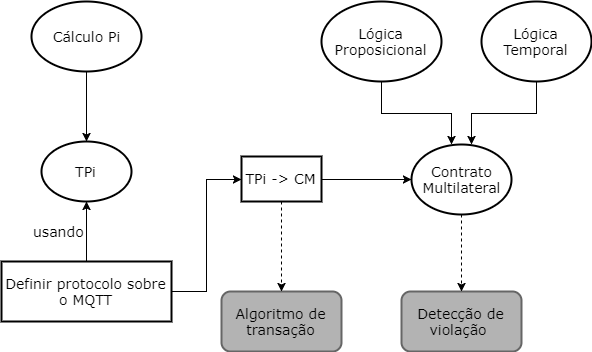
\includegraphics[width=1\textwidth]{imagens/tcc_estrutura.png}
	\caption{Escopo do método proposto.
		\label{fig:tcc_escopo}}
\end{figure}
\FloatBarrier

\section{Formulação e Escopo do Problema}

Como relatado acima, não se tem conhecimento de alguma ferramenta baseada em verificação formal que permita modelar a comunicação entre os dispositivos de projetos em IoT, assim como realizar a checagem automática de suas propriedades. Em vista disso, a principal questão a ser respondida é:

\textbf{É possível modelar e verificar a comunicação entre dispositivos que utilizam o protocolo MQTT?}

No intuito de responder essa questão, a resolução das seguintes subquestões devem ser fornecidas:

\textbf{\textit{(1) É possível modelar o MQTT?}}


No estudo desenvolvido por~\citeauthor{aziz2016formal}, e que serve de base para este trabalho, o protocolo é modelado através de uma álgebra temporal de processos, chamada \textit{TPi}.

\textbf{\textit{(2) É possível realizar a verificação formal do MQTT?}}

A partir do elaborado por~\citeauthor{aziz2016formal}, pode-se criar um algoritmo baseado em \textit{Model Checking} que faça a verificação de suas propriedades, o que leva ao objetivo do trabalho.

\section{Objetivos gerais e específicos}

